\documentclass[10pt]{beamer}\usepackage[]{graphicx}\usepackage[]{color}
%% maxwidth is the original width if it is less than linewidth
%% otherwise use linewidth (to make sure the graphics do not exceed the margin)
\makeatletter
\def\maxwidth{ %
  \ifdim\Gin@nat@width>\linewidth
    \linewidth
  \else
    \Gin@nat@width
  \fi
}
\makeatother

\definecolor{fgcolor}{rgb}{0.345, 0.345, 0.345}
\newcommand{\hlnum}[1]{\textcolor[rgb]{0.686,0.059,0.569}{#1}}%
\newcommand{\hlstr}[1]{\textcolor[rgb]{0.192,0.494,0.8}{#1}}%
\newcommand{\hlcom}[1]{\textcolor[rgb]{0.678,0.584,0.686}{\textit{#1}}}%
\newcommand{\hlopt}[1]{\textcolor[rgb]{0,0,0}{#1}}%
\newcommand{\hlstd}[1]{\textcolor[rgb]{0.345,0.345,0.345}{#1}}%
\newcommand{\hlkwa}[1]{\textcolor[rgb]{0.161,0.373,0.58}{\textbf{#1}}}%
\newcommand{\hlkwb}[1]{\textcolor[rgb]{0.69,0.353,0.396}{#1}}%
\newcommand{\hlkwc}[1]{\textcolor[rgb]{0.333,0.667,0.333}{#1}}%
\newcommand{\hlkwd}[1]{\textcolor[rgb]{0.737,0.353,0.396}{\textbf{#1}}}%
\let\hlipl\hlkwb

\usepackage{framed}
\makeatletter
\newenvironment{kframe}{%
 \def\at@end@of@kframe{}%
 \ifinner\ifhmode%
  \def\at@end@of@kframe{\end{minipage}}%
  \begin{minipage}{\columnwidth}%
 \fi\fi%
 \def\FrameCommand##1{\hskip\@totalleftmargin \hskip-\fboxsep
 \colorbox{shadecolor}{##1}\hskip-\fboxsep
     % There is no \\@totalrightmargin, so:
     \hskip-\linewidth \hskip-\@totalleftmargin \hskip\columnwidth}%
 \MakeFramed {\advance\hsize-\width
   \@totalleftmargin\z@ \linewidth\hsize
   \@setminipage}}%
 {\par\unskip\endMakeFramed%
 \at@end@of@kframe}
\makeatother

\definecolor{shadecolor}{rgb}{.97, .97, .97}
\definecolor{messagecolor}{rgb}{0, 0, 0}
\definecolor{warningcolor}{rgb}{1, 0, 1}
\definecolor{errorcolor}{rgb}{1, 0, 0}
\newenvironment{knitrout}{}{} % an empty environment to be redefined in TeX

\usepackage{alltt}
\usepackage{amsmath}
\usepackage{amssymb}
\usepackage{geometry}
\usepackage{graphicx}
\usepackage{url}
\usepackage{bm}

\makeatletter
\let \@sverbatim \@verbatim
\def \@verbatim {\@sverbatim \verbatimplus}
{\catcode`'=13 \gdef \verbatimplus{\catcode`'=13 \chardef '=13 }} 
\makeatother
\IfFileExists{upquote.sty}{\usepackage{upquote}}{}
\begin{document}

% --------------------------------------------
\begin{frame}
\large
Lecture 13:\\ 
Categorical Predictors and Interactions\\
STAT 632, Spring 2020\\
\end{frame}

% --------------------------------------------
\begin{frame}{Introduction}
\begin{itemize}
\item Predictors in a multiple linear regression model can either be \emph{quantitative} (e.g, weight, age) or \emph{qualitative} (e.g., gender, education level).  Qualitative predictors are also called \emph{categorical} or \emph{factors}.
\vspace{5pt}
\item A categorical predictor with two levels (0 or 1) is called a \emph{dummy} or \emph{indicator} variable.
\vspace{5pt}
\item Sometimes the effect that a quantitative predictor has on the response changes depending on the level of categorical predictor.  For example, perhaps the effect age has on salary depends on the education status of the person.  This is called an \emph{interaction} effect.
\end{itemize}
\end{frame}

% --------------------------------------------
\begin{frame}{Parallel Regression Lines}
Let $x$ be a quantitative variable, and $d$ a dummy variable.\\

\begin{align*}
Y = \beta_0 + \beta_1 x + \beta_2 d + e = 
\begin{cases}
\beta_0 + \beta_1 x + e, & \text{if d=0}\\
(\beta_0 + \beta_2) + \beta_1 x + e, & \text{if d=1}\\
\end{cases}
\end{align*}

\begin{itemize}
\item This model gives two separate regression lines that have the same slope but different intercepts.
\item The parameter $\beta_2$ represents the vertical distance between the two lines.
\end{itemize}
\end{frame}

% --------------------------------------------
\begin{frame}{Unrelated Regression Lines}
Let $x$ be a quantitative variable, and $d$ a dummy variable.\\

\begin{align*}
Y &= \beta_0 + \beta_1 x + \beta_2 d + \beta_3 d \cdot x + e\\ 
& = \begin{cases}
\beta_0 + \beta_1 x + e, & \text{if d=0}\\
(\beta_0 + \beta_2) + (\beta_1 + \beta_3) x + e, & \text{if d=1}\\
\end{cases}
\end{align*}

\begin{itemize}
\item This model gives two separate regression lines that have different slopes, and different intercepts.
\item $\beta_3$ is the coefficient for the \emph{interaction} between the dummy variable, $d$, and the quantitative variable, $x$.  
\end{itemize}
\end{frame}

% --------------------------------------------
\begin{frame}[fragile]{Example: Credit Card Data Set}
\begin{itemize}
\item We consider the \texttt{Credit} data set from the \texttt{ISLR} package.  Type \texttt{help(Credit)} to read about this data set in the help menu.\\
\vspace{5pt}
\item The response variable is \texttt{Balance}, the average credit card balance in dollars.\\
\vspace{5pt}
\item The predictors of interest are \texttt{Income} (in thousands of dollars) and \texttt{Student}, a dummy variable indicating student status (No $=0$ or Yes $=1$).
\end{itemize}
\scriptsize
\begin{verbatim}
> library(ISLR)
> head(Credit, n=5)
  ID  Income Limit Rating Cards Age Education Gender Student Married Ethnicity Balance
1  1  14.891  3606    283     2  34        11   Male      No     Yes Caucasian     333
2  2 106.025  6645    483     3  82        15 Female     Yes     Yes     Asian     903
3  3 104.593  7075    514     4  71        11   Male      No      No     Asian     580
4  4 148.924  9504    681     3  36        11 Female      No      No     Asian     964
5  5  55.882  4897    357     2  68        16   Male      No     Yes Caucasian     331
\end{verbatim}
\end{frame}

% --------------------------------------------
\begin{frame}[fragile]
\small
\begin{verbatim}
> lm1 <- lm(Balance ~ Income + Student, data=Credit)

# shows coding R uses for the dummy variable
> contrasts(Credit$Student) 
    Yes
No    0
Yes   1

> summary(lm1)
Coefficients:
            Estimate Std. Error t value Pr(>|t|)    
(Intercept) 211.1430    32.4572   6.505 2.34e-10 ***
Income        5.9843     0.5566  10.751  < 2e-16 ***
StudentYes  382.6705    65.3108   5.859 9.78e-09 ***
---
Signif. codes:  0 ‘***’ 0.001 ‘**’ 0.01 ‘*’ 0.05 ‘.’ 0.1 ‘ ’ 1

Residual standard error: 391.8 on 397 degrees of freedom
Multiple R-squared:  0.2775,	Adjusted R-squared:  0.2738 
F-statistic: 76.22 on 2 and 397 DF,  p-value: < 2.2e-16
\end{verbatim}
\end{frame}

% --------------------------------------------
\begin{frame}
We can write the regression equation for the fit:
\begin{align*}
\widehat{\texttt{Balance}} &= \hat{\beta}_0 + \hat{\beta}_1 \texttt{income} + \hat{\beta}_2 \texttt{student} =\\ 
&= \begin{cases}
\hat{\beta}_0 + \hat{\beta}_1 \texttt{income}, & \text{if \texttt{student}=0 (No)}\\
(\hat{\beta}_0 + \hat{\beta}_2) + \hat{\beta}_1 \texttt{income}, & \text{if \texttt{student}=1 (Yes)}\\
\end{cases}
\end{align*}
\vspace{10pt}

Plugging in the coefficients from the regression summary gives:
\begin{align*}
\widehat{\texttt{Balance}} &= 211.14 + 5.98 \texttt{income} + 382.67 \texttt{student} =\\ 
&= \begin{cases}
211.14 + 5.98 \texttt{income}, & \text{if \texttt{student}=0 (No)}\\
593.81 + 5.98 \texttt{income}, & \text{if \texttt{student}=1 (Yes)}\\
\end{cases}
\end{align*}
\end{frame}

% --------------------------------------------
\begin{frame}[fragile]
\small
\begin{verbatim}
ggplot(Credit, aes(Income, Balance, colour = Student)) +
  geom_point(alpha=0.7) +
  geom_abline(intercept = 211.1, slope = 5.98, colour = "#F8766D") +
  geom_abline(intercept = 593.8, slope = 5.98, colour = "#00BFC4")
\end{verbatim}
\begin{figure}
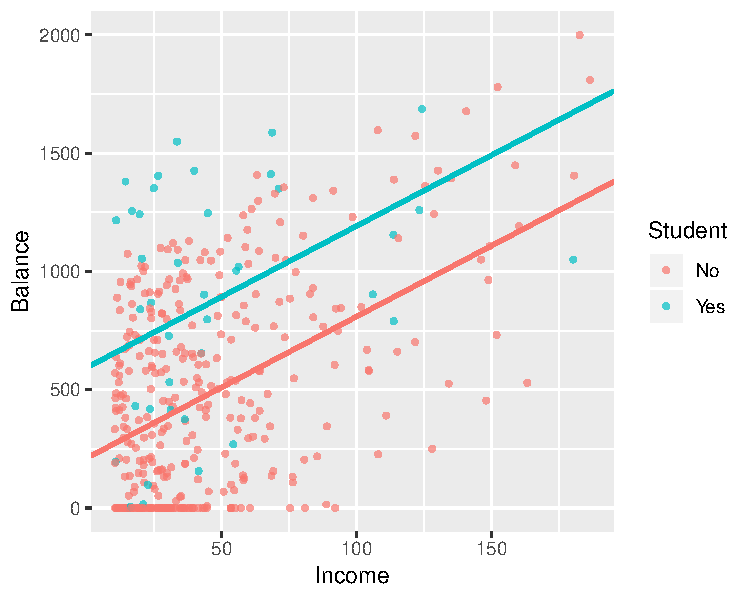
\includegraphics[scale=0.6]{figure/balance_parallel.pdf}
\end{figure}
\end{frame}

% --------------------------------------------
\begin{frame}[fragile]
\small
\begin{verbatim}
> lm2 <- lm(Balance ~ Income + Student + Income:Student, data=Credit)
> summary(lm2)

Coefficients:
                  Estimate Std. Error t value Pr(>|t|)    
(Intercept)       200.6232    33.6984   5.953 5.79e-09 ***
Income              6.2182     0.5921  10.502  < 2e-16 ***
StudentYes        476.6758   104.3512   4.568 6.59e-06 ***
Income:StudentYes  -1.9992     1.7313  -1.155    0.249    
---
Signif. codes:  0 ‘***’ 0.001 ‘**’ 0.01 ‘*’ 0.05 ‘.’ 0.1 ‘ ’ 1

Residual standard error: 391.6 on 396 degrees of freedom
Multiple R-squared:  0.2799,	Adjusted R-squared:  0.2744 
F-statistic:  51.3 on 3 and 396 DF,  p-value: < 2.2e-16
\end{verbatim}
\end{frame}

% --------------------------------------------
\begin{frame}[fragile]
We can write the regression equation for the fit:
\begin{align*}
\widehat{\texttt{Balance}} &= \hat{\beta}_0 + \hat{\beta}_1 \texttt{income} + \hat{\beta}_2 \texttt{student} 
+ \hat{\beta}_3 \texttt{student} \cdot \texttt{income}\\ 
& = \begin{cases}
\hat{\beta}_0 + \hat{\beta}_1 \texttt{income}, & \text{if \texttt{student}=0 (No)}\\
(\hat{\beta}_0 + \hat{\beta}_2) + (\hat{\beta}_1 + \hat{\beta}_3) \texttt{income}, & \text{if \texttt{student}=1 (Yes)}\\
\end{cases}
\end{align*}
\vspace{5pt}

Plugging in the coefficients from the regression summary gives:
\begin{align*}
\widehat{\texttt{Balance}} &= 200.62 + 6.22 \texttt{income} + 476.68 \texttt{student} 
- 2.00 \texttt{student} \cdot \texttt{income}\\ 
& = \begin{cases}
200.62 + 6.22\texttt{income}, & \text{if \texttt{student}=0 (No)}\\
677.3 + 4.22 \texttt{income}, & \text{if \texttt{student}=1 (Yes)}\\
\end{cases}
\end{align*}
\vspace{5pt}

Note that the coefficient for the interaction, $\beta_3$, is not significant ($p$-value$ = 0.249$), so we do not necessarily need to include the interaction term.
\end{frame}

% --------------------------------------------
\begin{frame}[fragile]
\small
\begin{verbatim}
ggplot(Credit, aes(Income, Balance, colour = Student)) +
  geom_point(alpha=0.7) +
  geom_smooth(method="lm", se=FALSE)
\end{verbatim}
\begin{figure}
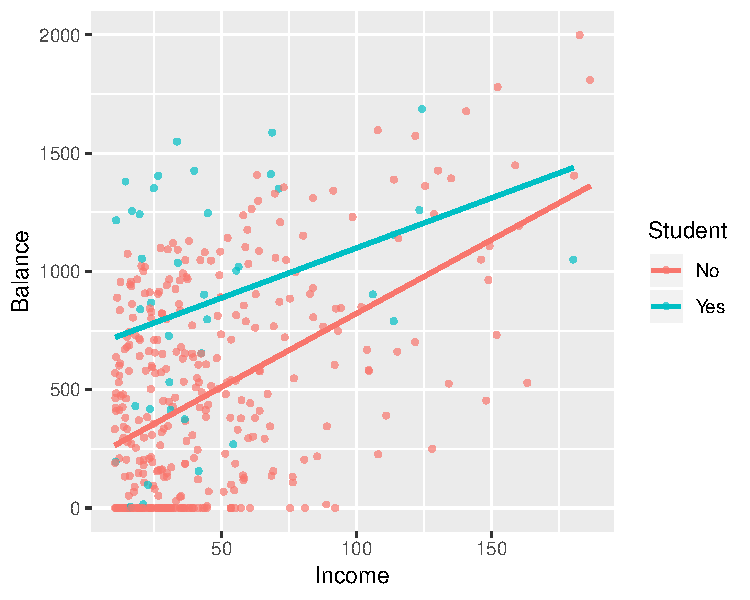
\includegraphics[scale=0.6]{figure/balance_unrelated.pdf}
\end{figure}
\end{frame}

% --------------------------------------------
\begin{frame}{Categorical Predictors with More Than Two Levels}
\begin{itemize}
\item When a categorical predictor contains more than two levels, we create additional dummy variables.\\
\vspace{5pt}
\item For example, consider the \texttt{Wage} data set also from the \texttt{ISLR} package.  The data contain information on 3000 males workers in the Mid-Atlantic region.\\
\vspace{5pt}
\item The response variable is \texttt{logwage}, the log of the workers wage.\\
\vspace{5pt}
\item The predictor \texttt{education} is a categorical variable indicating education level with 5 levels: 1. $<$ HS Grad, 2. HS Grad, 3. Some College, 4. College Grad, and 5. Advanced Degree.
\end{itemize}
\end{frame}

% --------------------------------------------
\begin{frame}
We can write the regression equation with 4 dummy variables:
\begin{align*}
\log(\texttt{Wage}) &= \beta_0 + \beta_1 \texttt{HS\_Grad} + \beta_2 \texttt{Some\_College}\\ 
& \quad + \beta_3 \texttt{College\_Grad} + \beta_4 \texttt{Advanced\_Degree} + e\\
& = \begin{cases}
\beta_0 + e & \text{if  \texttt{<HS\_Grad} (baseline)}\\
\beta_0 + \beta_1 + e & \text{if \texttt{HS\_Grad}  = 1}\\
\beta_0 + \beta_2 + e & \text{if \texttt{Some\_College}  = 1}\\
\beta_0 + \beta_3 + e & \text{if \texttt{College\_Grad}  = 1}\\
\beta_0 + \beta_4 + e & \text{if \texttt{Advanced\_Degree}  = 1}
\end{cases}
\end{align*}
In general, if we have a categorical variable with $k$ levels, then the regression equation contains $k-1$ dummy variables. 
\end{frame}

% --------------------------------------------
\begin{frame}[fragile]
\small
\begin{verbatim}
ggplot(Wage, aes(education, logwage)) + 
  geom_boxplot() + coord_flip()
\end{verbatim}
\begin{figure}
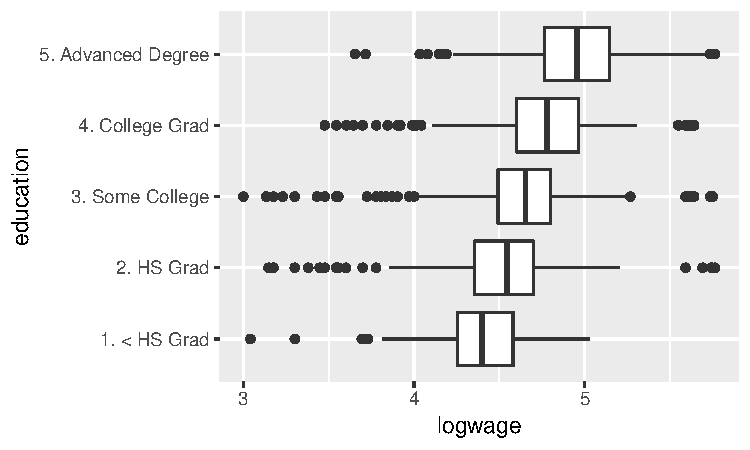
\includegraphics[scale=0.7]{figure/educ_boxplots.pdf}
\end{figure}
\end{frame}

% --------------------------------------------
\begin{frame}[fragile]
\small
\begin{verbatim}
> lm1 <- lm(logwage ~ education, data=Wage)
> summary(lm1)

Coefficients:
                            Estimate Std. Error t value Pr(>|t|)    
(Intercept)                  4.39759    0.01891 232.502  < 2e-16 ***
education2. HS Grad          0.12295    0.02137   5.754 9.57e-09 ***
education3. Some College     0.23821    0.02248  10.597  < 2e-16 ***
education4. College Grad     0.37373    0.02231  16.752  < 2e-16 ***
education5. Advanced Degree  0.56036    0.02414  23.212  < 2e-16 ***
---
Signif. codes:  0 ‘***’ 0.001 ‘**’ 0.01 ‘*’ 0.05 ‘.’ 0.1 ‘ ’ 1

Residual standard error: 0.3096 on 2995 degrees of freedom
Multiple R-squared:  0.2262,	Adjusted R-squared:  0.2251 
F-statistic: 218.8 on 4 and 2995 DF,  p-value: < 2.2e-16
\end{verbatim}
\end{frame}

% --------------------------------------------
\begin{frame}[fragile]
Using the summary output we can write the fitted regression model as
\begin{align*}
\widehat{\log(\texttt{Wage})} &=  4.398 + 0.123 \texttt{HS\_Grad} + 0.238 \texttt{Some\_College}\\ 
& \quad + 0.374 \texttt{College\_Grad} + 0.560 \texttt{Advanced\_Degree}\\
& = \begin{cases}
4.398 & \text{if  \texttt{<HS\_Grad} (baseline)}\\
4.398 + 0.123 = 4.521  & \text{if \texttt{HS\_Grad}  = 1}\\
4.398 + 0.238 = 4.636 & \text{if \texttt{Some\_College}  = 1}\\
4.398 + 0.374 = 4.772  & \text{if \texttt{College\_Grad}  = 1}\\
4.398 + 0.560 = 4.958 & \text{if \texttt{Advanced\_Degree}  = 1}
\end{cases}
\end{align*}
\end{frame}

% --------------------------------------------
\begin{frame}
We can also include interaction effects between the categorical predictor $\texttt{education}$ and a quantitative variable such as $\texttt{age}$ (age of worker).  The model can be written out as:
\small 
\begin{align*}
\log(\texttt{Wage}) &= \beta_0 + \beta_1 \texttt{age} 
+ \beta_2 \texttt{HS\_Grad} + \beta_3 \texttt{Some\_College}\\ 
& \quad + \beta_4 \texttt{College\_Grad} +\beta_5 \texttt{Advanced\_Degree}\\ 
& \quad + \beta_6 \texttt{HS\_Grad} \cdot \texttt{age}
+ \beta_7 \texttt{Some\_College} \cdot \texttt{age}\\
& \quad + \beta_8 \texttt{College\_Grad} \cdot \texttt{age}
+ \beta_9 \texttt{Advanced\_Degree} \cdot \texttt{age} + e\\
&= \begin{cases}
\beta_0 + \beta_1 \texttt{age} + e & \text{if  \texttt{<HS\_Grad} (baseline)}\\
\beta_0 + \beta_2 + (\beta_1 + \beta_6) \texttt{age} + e & \text{if \texttt{HS\_Grad}  = 1}\\
\beta_0 + \beta_3 + (\beta_1 + \beta_7) \texttt{age} + e & \text{if \texttt{Some\_College}  = 1}\\
\beta_0 + \beta_4 + (\beta_1 + \beta_8) \texttt{age} + e & \text{if \texttt{College\_Grad}  = 1}\\
\beta_0 + \beta_5 + (\beta_1 + \beta_9) \texttt{age} + e & \text{if \texttt{Advanced\_Degree}  = 1}
\end{cases}
\end{align*}
The regression model gives separate regression lines, which have different slopes and intercepts, for each level of the categorical predictor \texttt{education}.
\end{frame}

% --------------------------------------------
\begin{frame}[fragile]
\scriptsize
\begin{verbatim}
> lm3 <- lm(logwage ~ age + education + age:education, data=Wage)
> summary(lm3)

Coefficients:
                                  Estimate Std. Error t value Pr(>|t|)    
(Intercept)                      4.1921197  0.0640086  65.493  < 2e-16 ***
age                              0.0049162  0.0014664   3.353 0.000811 ***
education2. HS Grad              0.0979291  0.0731558   1.339 0.180791    
education3. Some College         0.0644316  0.0775180   0.831 0.405937    
education4. College Grad         0.4160484  0.0792801   5.248 1.65e-07 ***
education5. Advanced Degree      0.6467308  0.0918866   7.038 2.40e-12 ***
age:education2. HS Grad          0.0005434  0.0016738   0.325 0.745466    
age:education3. Some College     0.0043591  0.0017917   2.433 0.015033 *  
age:education4. College Grad    -0.0011018  0.0018093  -0.609 0.542593    
age:education5. Advanced Degree -0.0022699  0.0020470  -1.109 0.267563    
---
Signif. codes:  0 ‘***’ 0.001 ‘**’ 0.01 ‘*’ 0.05 ‘.’ 0.1 ‘ ’ 1

Residual standard error: 0.3022 on 2990 degrees of freedom
Multiple R-squared:  0.2642,	Adjusted R-squared:  0.262 
F-statistic: 119.3 on 9 and 2990 DF,  p-value: < 2.2e-16
\end{verbatim}
\end{frame}

\begin{frame}[fragile]
\small
\begin{verbatim}
ggplot(Wage, aes(age, logwage)) +
  geom_point(size = 0.3, alpha=0.6) + facet_wrap( ~ education) +
  geom_smooth(method='lm')
\end{verbatim}
\begin{figure}
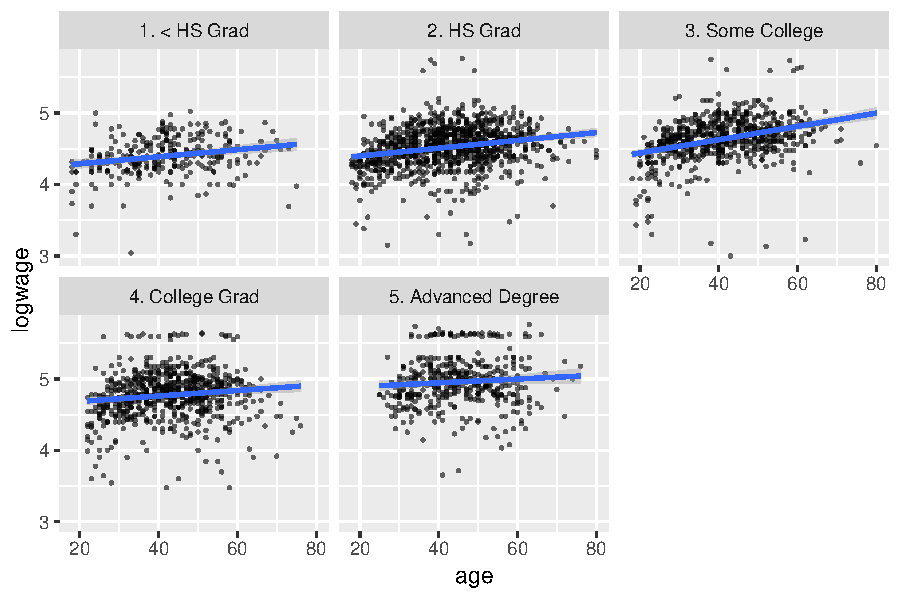
\includegraphics[scale=0.65]{figure/educ_age_lm_scatter.pdf}
\end{figure}
\end{frame}

% --------------------------------------------
\begin{frame}[fragile]
To determine whether the interaction effects are actually meaningful to include we can use a model selection criteria such as adjusted $R^2$.

\small
\begin{verbatim}
> lm1 <- lm(logwage ~ education, data=Wage)
> summary(lm1)$adj.r.squared
[1] 0.2251165
> lm2 <- lm(logwage ~ age + education, data=Wage)
> summary(lm2)$adj.r.squared
[1] 0.2580081
> lm3 <- lm(logwage ~ age + education + age:education, data=Wage)
> summary(lm3)$adj.r.squared
[1] 0.261979
\end{verbatim}
We see that the model \texttt{lm3} with \texttt{age}, \texttt{education}, and the interaction effects between \texttt{age} and \texttt{education} is the best fitting model according to the adjusted $R^2$.
\end{frame}

% --------------------------------------------
\begin{frame}[fragile]
The F-test can also be used to compare the nested models.  For example we can test whether or not $H_0: \beta_6 = \cdots = \beta_9 = 0$ (the coefficients for the interaction terms are all zero).
\begin{verbatim}
> anova(lm2, lm3)
Analysis of Variance Table

Model 1: logwage ~ age + education
Model 2: logwage ~ age + education + age:education
  Res.Df    RSS Df Sum of Sq      F    Pr(>F)    
1   2994 274.87                                  
2   2990 273.03  4    1.8363 5.0273 0.0004885 ***
---
Signif. codes:  0 ‘***’ 0.001 ‘**’ 0.01 ‘*’ 0.05 ‘.’ 0.1 ‘ ’ 1
\end{verbatim}
Since the $p$-value$< 0.001$ we reject $H_0$, which means that the model with the interactions is superior.  This agrees with the adjusted $R^2$ criteria.
\end{frame}

% --------------------------------------------
\begin{frame}[fragile]
\small
\emph{An aside} - \texttt{ggplot2} can also be used to investigate nonlinear relationships in the data.  Below we add a loess smoother to each scatter plot.\footnote{See ISLR, Ch. 7, pp. 280-282 to learn more about local regression.}

\begin{verbatim}
ggplot(Wage, aes(age, logwage)) +
  geom_point(size = 0.3, alpha=0.6) + facet_wrap( ~ education) +
  geom_smooth(method='loess')
\end{verbatim}
\begin{figure}
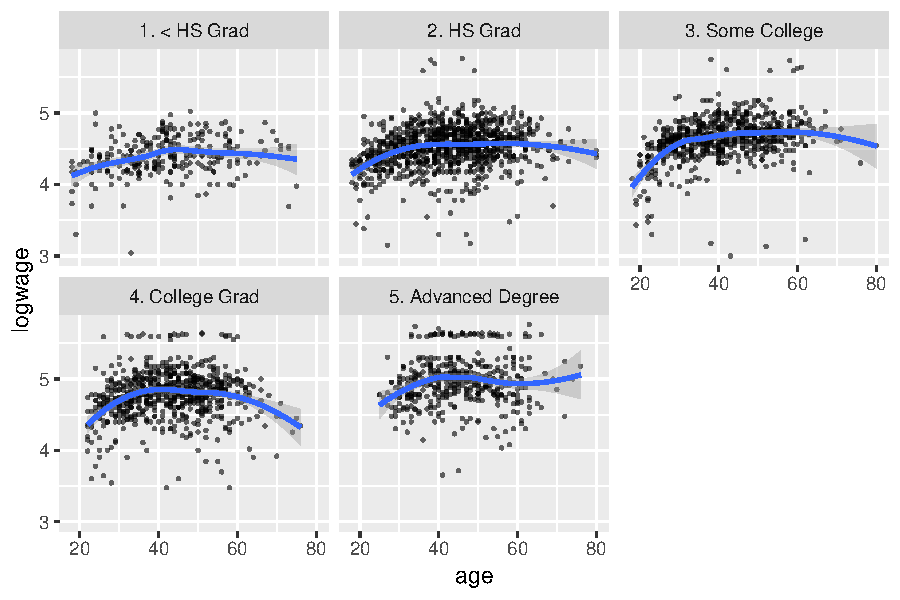
\includegraphics[scale=0.55]{figure/educ_age_loess_scatter.pdf}
\end{figure}
\end{frame}

\end{document}
